\scanpage{58}
\figure{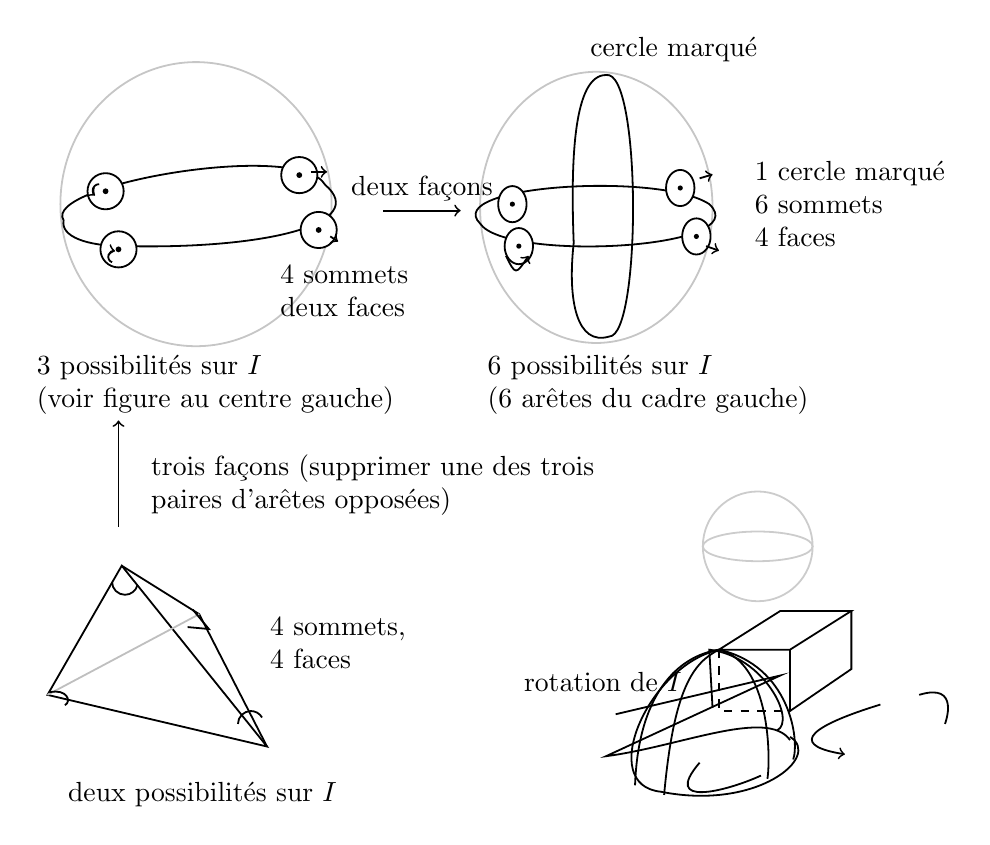
\begin{tikzpicture}[x=0.82cm,y=0.82cm,line width=.65pt]
\draw[gray!45] (2.3,8.7) ellipse (2.1 and 2.2);
\draw (0.25,8.45) .. controls (-.1,9) and (3.9,9.7) .. (4.3,9) .. controls (5,8.4) and (3.4,8) .. (1.2,8.05) .. controls (.6,8.05) and (.2,8.2) .. (.25,8.45);
\foreach \x/\y in {.9/8.9,1.1/8.0,3.9/9.15,4.2/8.3}{\draw[fill=white] (\x,\y) circle (.28);\fill (\x,\y) circle (.045);}
\draw[->] (.8,9.01) arc (90:230:.10);\draw[->] (1,7.8) arc (250:80:.09);\draw[->] (4.08,9.2)--(4.33,9.2);\draw[->] (4.38,8.2)--(4.5,8.12);
\node[align=left,anchor=west] at (3.45,7.35) {4 sommets\\deux faces};
\draw[->] (5.2,8.6)--(6.4,8.6) node[midway,above]{deux façons};
\draw[gray!45] (8.5,8.65) ellipse (1.8 and 2.1);
\draw (6.7,8.4) .. controls (6.1,9) and (9.5,9.2) .. (10.25,8.7) .. controls (11,8) and (7.1,7.8) .. (6.7,8.4);
\draw (8.15,8.1) .. controls (8.1,9.4) and (8.15,10.7) .. (8.65,10.7) .. controls (9.2,10.8) and (9.2,6.65) .. (8.7,6.65) .. controls (8.2,6.5) and (8.05,7.2) .. (8.15,8.1);
\foreach \x/\y in {7.2/8.7,7.3/8.05,9.8/8.95,10.05/8.2}{\draw[fill=white] (\x,\y) ellipse (.22 and .28);\fill (\x,\y) circle (.04);}
\draw[->] (7.1,7.9)..controls(7.25,7.6)..(7.45,7.9);\draw[->] (10.1,9.1)--(10.3,9.16);\draw[->](10.2,8.05)--(10.4,7.98);
\node at (9.7,11.1){\deleted{cercle marqué}};
\node[align=left,anchor=west] at (10.8,8.7){1 cercle marqué\\6 sommets\\4 faces};
\node[align=left] at (2.6,5.9){\uline{3 possibilités} sur $I$\\(\unsure{voir figure au centre gauche})};
\node[align=left] at (9.3,5.9){6 possibilités sur $I$\\(\unsure{6 arêtes du cadre gauche})};
\draw[->] (1.1,3.7)--(1.1,5.35);
\node[align=left,anchor=west] at (1.45,4.35){trois façons (supprimer une des trois\\\deleted{\unsure{paires}} d'arêtes opposées)};
\draw (0,1.1)--(1.15,3.1)--(3.4,.3)--cycle;
\draw (1.15,3.1)--(2.35,2.35)--(3.4,.3);\draw[gray!50](0,1.1)--(2.35,2.35);
\draw (1,2.85) arc(180:345:.2);\draw (2.17,2.15)--(2.5,2.12)--(2.25,2.42);\draw(.03,1.14)..controls(.3,1.2)and(.38,1)..(.27,.94);\draw(2.95,.65) arc(180:30:.2);
\node[align=left] at (4.5,1.9){4 sommets,\\4 faces};
\node at (2.4,-.45){deux possibilités sur $I$};
\draw[gray!40] (11,3.4) circle (.85);\draw[gray!40](11,3.4) ellipse(.85 and .23);
\draw (10.4,1.8)--(11.35,2.4)--(12.45,2.4)--(11.5,1.8)--cycle;\draw(11.5,1.8)--(11.5,.85)--(12.45,1.5)--(12.45,2.4);\draw[dashed](10.4,1.8)--(10.4,.85)--(11.5,.85);
\draw (10.4,1.8)..controls(9.3,1.55)and(8.5,-.3)..(9.5,-.4)..controls(11,-.7)and(12,.15)..(11.5,.45);
\draw(9.1,-.3)..controls(9.15,1.1)and(9.75,1.7)..(10.4,1.8)..controls(11.2,1.6)and(11.2,.1)..(11.15,-.2);
\draw(9.55,-.45)..controls(9.7,1.2)and(10,1.6)..(10.4,1.8)..controls(11.5,1.55)and(11.65,.4)..(11.55,.1);
\draw(10.3,.9)--(10.25,1.8)..controls(11.1,1.7)and(11.6,.7)..(11.3,.55);
\draw(8.8,.8)--(11.35,1.4)--(8.65,.15)..controls(9.8,.3)and(11.15,.9)..(11.5,.4);
\draw(10.1,.05)..controls(9.5,-.65)and(10.5,-.4)..(11.05,-.15);
\draw[->](12.9,.95)..controls(11.6,.55)and(11.6,.3)..(12.35,.18);\draw(13.5,1.1)..controls(14.15,1.3)and(13.9,.65)..(13.9,.65);
\node at (8.6,1.3){\deleted{\unsure{rotation de $I$}}};
\end{tikzpicture}}

\figure{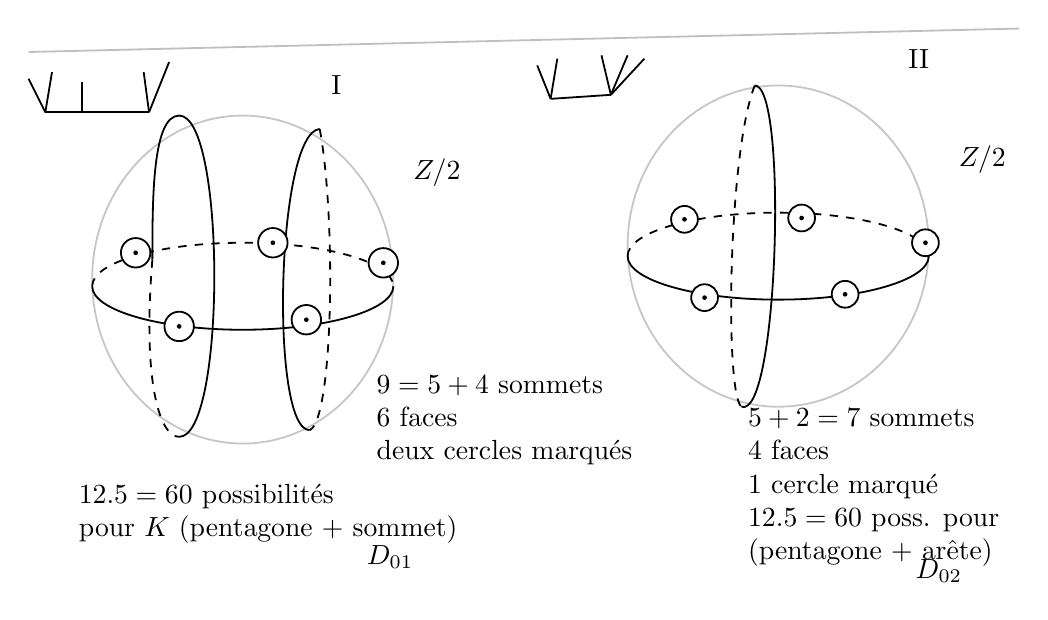
\begin{tikzpicture}[x=.85cm,y=.85cm,line width=.65pt]
\draw[gray!50](-.6,5.7)--(14.2,6.05);
\node at (4,5.2){I};\node at (12.7,5.6){II};
\draw(-.35,4.8)--(.6,4.8)--(1.2,4.8);\draw(-.35,4.8)--(-.6,5.3);\draw(-.35,4.8)--(-.25,5.4);\draw(.2,4.8)--(.2,5.25);\draw(1.2,4.8)--(1.12,5.4);\draw(1.2,4.8)--(1.5,5.55);
\draw(7.2,5)--(8.1,5.06);\draw(7.2,5)--(7,5.5);\draw(7.2,5)--(7.3,5.6);\draw(8.1,5.06)--(7.96,5.65);\draw(8.1,5.06)--(8.35,5.65);\draw(8.1,5.06)--(8.6,5.6);
\draw[gray!45] (2.6,2.3) ellipse(2.25 and 2.45);\draw (0.35,2.2) arc(180:360:2.25 and .65);\draw[dashed](.35,2.2) arc(180:0:2.25 and .65);
\draw(1.65,-.05)..controls(2.35,-.05)and(2.35,4.75)..(1.65,4.75)..controls(1.25,4.75)and(1.25,3.5)..(1.25,2.6);\draw[dashed](1.25,2.6)..controls(1.1,.8)and(1.35,-.05)..(1.65,-.05);
\draw(3.6,.05)..controls(3,.05)and(3.1,4.5)..(3.75,4.55);\draw[dashed](3.75,4.55)..controls(4,3.2)and(3.95,.2)..(3.6,.05);
\foreach \x/\y in {1/2.7,1.65/1.6,3.05/2.85,3.55/1.7,4.7/2.55}{\draw[fill=white](\x,\y) circle(.22);\fill(\x,\y)circle(.035);}
\node at (5.5,3.9){$\mathbb Z/2$};
\node[align=left,anchor=west] at (4.45,.2){$9=5+4$ sommets\\6 faces\\deux cercles marqués};
\node[align=left,anchor=west] at (0,-1.2){$12.5=\uline{60}$ possibilités\\pour $K$ (pentagone + sommet)};
\node at (4.8,-1.85){$D_{01}$};
\draw[gray!45](10.6,2.8) ellipse(2.25 and 2.4);\draw(8.35,2.65) arc(180:360:2.25 and .65);\draw[dashed](8.35,2.65) arc(180:0:2.25 and .65);
\draw(10.05,.4)..controls(10.6,.2)and(10.75,5.2)..(10.25,5.2);\draw[dashed](10.25,5.2)..controls(9.85,4.2)and(9.8,.6)..(10.05,.4);
\foreach \x/\y in {9.2/3.2,9.5/2.03,10.95/3.22,11.6/2.08,12.8/2.85}{\draw[fill=white](\x,\y)circle(.2);\fill(\x,\y)circle(.035);}
\node at (13.65,4.1){$\mathbb Z/2$};
\node[align=left,anchor=west] at (10,-.3){$5+2=7$ sommets\\4 faces\\1 cercle marqué};
\node[align=left,anchor=west] at (10,-1.55){$12.5=60$ poss. pour\\(pentagone + arête)};
\node at (13,-2.05){$D_{02}$};
\end{tikzpicture}}
\mspage{57}
